\scanpage{124}
On aura évidemment
\[
t_{ij}=\varepsilon_{ij}f_{ij}^{n_i}=\varepsilon_{ji}f_{ji}^{n_j}
\]
\inserted{$\unsure{\varepsilon''_{ij}}f^{n_i}=\varepsilon_{ji}f^{n_j}$}

\deleted{Supp Je dis que} \deleted{\unsure{Supp}} Je dis que $n_i=n_j$. Supposons en effet $n_i>n_j$, on aurait \deleted{$(\varepsilon_{ij}/\varepsilon_{ji})f_{ij}^{n_i-n_j}=1$,} \deleted{et comme}
\[
f_{ij}^{(n_i-n_j)}=\varepsilon_{ji}/\varepsilon_{ij}
\]
donc $f_{ij}$ serait une unité, ce qui \deleted{n'est pas le cas} est absurde puisque $f_{ij}$ s'annule sur $Z_{ij}\subset X_{ij}$.

\margin{\figure{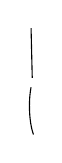
\begin{tikzpicture}[x=0.3cm,y=0.3cm]\draw (0,4.5)--(0.05,2.4);\draw (0,2.0) .. controls (-0.12,1.4) and (-0.08,0.5) .. (0.1,0);\end{tikzpicture}}}
\uline{Théorème}. Soit $f:X\text{---}Y$ un morphisme propre \inserted{et} \uline{séparable}, \inserted{$Y$ loc. noeth. On suppose que $X/Y$ \unsure{0-coh. universellement} \unsure{pour} tt $Y'\leftarrow Y$} \deleted{On suppose que} $n(y)$ le nb des composantes irréductibles \uline{absolues} de $f^{-1}(y)$, et supposons $n(y)$ loc. constant. Soit $\underline L$ un faisceau inversible sur $X$. \deleted{Alors} \inserted{\unsure{On a (i)|On a}} Il existe un plus \unsure{grand} sous-préschéma \deleted{\unsure{fermé}} fermé $Y'$ de $Y$ tel que $\underline L\otimes_Y Y'$ soit isomorphe au faisceau trivial sur $Y$, \unsure{ce est} \deleted{\unsure{appelé}} $S(L/X/Y)$.

(ii) On a.
\[
S(\unsure{L_1^a},X_1,Y_1)\simeq S(L/X/Y)\times_Y Y_1
\]
\margin{123}
